\subsection{Db\-Image\-List  Class Reference}
\label{class_dbimagelist}\index{DbImageList@{Db\-Image\-List}}
Db\-Images can be globally located and stored into image lists. 


{\tt \#include $<$dbimage.h$>$}

Inheritance diagram for Db\-Image\-List::\begin{figure}[H]
\begin{center}
\leavevmode
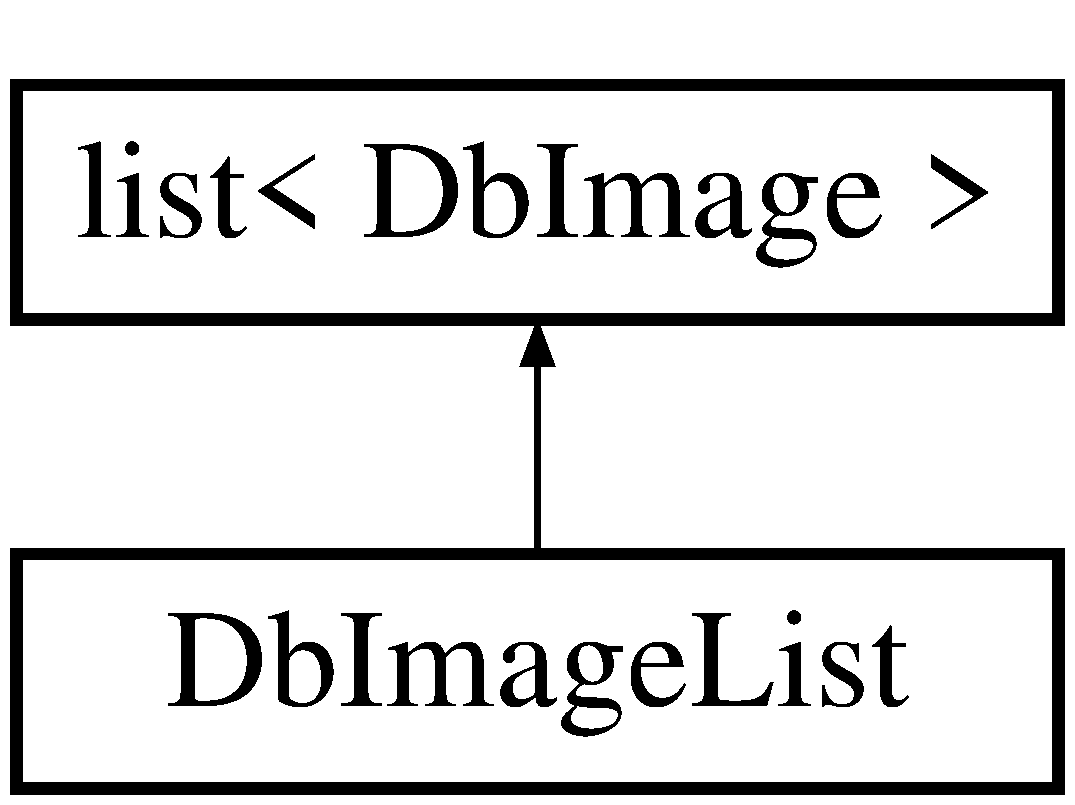
\includegraphics[height=2cm]{class_dbimagelist}
\end{center}
\end{figure}
\subsubsection*{Public Methods}
\begin{CompactItemize}
\item 
{\bf Db\-Image\-List} (const char $\ast$Path\-Name)
\begin{CompactList}\small\item\em locates all {\bf Db\-Image} {\rm (p.\,\pageref{class_dbimage})}'s in a given symbolic path name (see db configuration file section).\item\end{CompactList}\item 
\index{DbImageList@{DbImageList}!DbImageList@{Db\-Image\-List}}\index{DbImageList@{DbImageList}!DbImageList@{Db\-Image\-List}}
{\bf Db\-Image\-List} (const string \&Path\-Name)\label{class_dbimagelist_a1}

\item 
\index{DbImageList@{DbImageList}!DbImageList@{Db\-Image\-List}}\index{DbImageList@{DbImageList}!DbImageList@{Db\-Image\-List}}
{\bf Db\-Image\-List} (const list$<$ string $>$ names)\label{class_dbimagelist_a2}

\begin{CompactList}\small\item\em tries to interpret ecah argument either as a {\bf Db\-Image} {\rm (p.\,\pageref{class_dbimage})} name or as a symbolic path.\item\end{CompactList}\item 
\index{DbImageList@{DbImageList}!DbImageList@{Db\-Image\-List}}\index{DbImageList@{DbImageList}!DbImageList@{Db\-Image\-List}}
{\bf Db\-Image\-List} ()\label{class_dbimagelist_a3}

\item 
\index{FilterByDate@{FilterByDate}!DbImageList@{Db\-Image\-List}}\index{DbImageList@{DbImageList}!FilterByDate@{Filter\-By\-Date}}
void {\bf Filter\-By\-Date} (const int a\_\-date)\label{class_dbimagelist_a4}

\begin{CompactList}\small\item\em discards from a Db\-Image\-List all images not matching a date.\item\end{CompactList}\item 
\index{Collect@{Collect}!DbImageList@{Db\-Image\-List}}\index{DbImageList@{DbImageList}!Collect@{Collect}}
int {\bf Collect} (const char $\ast$Path\-Name)\label{class_dbimagelist_a5}

\begin{CompactList}\small\item\em DOCF collects and appends Db\-Images inside Path\-Name.\item\end{CompactList}\item 
\index{dump@{dump}!DbImageList@{Db\-Image\-List}}\index{DbImageList@{DbImageList}!dump@{dump}}
void {\bf dump} (ostream \&stream=cout) const\label{class_dbimagelist_a6}

\end{CompactItemize}
\subsubsection*{Friends}
\begin{CompactItemize}
\item 
\index{operator<<@{operator$<$$<$}!DbImageList@{Db\-Image\-List}}\index{DbImageList@{DbImageList}!operator<<@{operator$<$$<$}}
ostream\& {\bf operator$<$$<$} (ostream \&stream, const Db\-Image\-List \&L)\label{class_dbimagelist_l0}

\begin{CompactList}\small\item\em example of usage : cout $<$$<$ Db\-Image\-List(\char`\"{}$\ast$\char`\"{}); . It works as the first statement of your program !\item\end{CompactList}\end{CompactItemize}


\subsubsection{Detailed Description}
Db\-Images can be globally located and stored into image lists.



\subsubsection{Constructor \& Destructor Documentation}
\index{DbImageList@{Db\-Image\-List}!DbImageList@{DbImageList}}
\index{DbImageList@{DbImageList}!DbImageList@{Db\-Image\-List}}
\paragraph{\setlength{\rightskip}{0pt plus 5cm}Db\-Image\-List::Db\-Image\-List (const char $\ast$ {\em Path\-Name})}\hfill\label{class_dbimagelist_a0}


locates all {\bf Db\-Image} {\rm (p.\,\pageref{class_dbimage})}'s in a given symbolic path name (see db configuration file section).

This routine handles wildcards : $\ast$ will match any path name, 'new$\ast$' will match any path name beginning with 'new'. 

The documentation for this class was generated from the following file:\begin{CompactItemize}
\item 
{\bf dbimage.h}\end{CompactItemize}
